\section{Novel intensifier length increases strength of interpretation}

Although the meanings of our existing English intensifiers could have influenced their lengths and frequencies over time, novel intensifiers have no meaning already associated with them. Therefore, if we found a relationship between the length of a novel intensifier and its interpreted meaning, we would have evidence that length can causally influence meaning. In the following two experiments, we directly manipulate the lengths of novel intensifiers and show that longer novel intensifiers are interpreted as having stronger meanings.

\subsection{Study 3 \label{sec:study3}}

In Study~\hyperref[sec:study3]{3} we show that longer novel intensifiers are interpreted as having stronger meanings, using our dependent measure from Study~\hyperref[sec:study1a]{1a}.

\subsubsection{Method}

\paragraph{Participants}

30 participants with US IP addresses were recruited through Amazon's Mechanical Turk and paid \$0.80 for their participation. 2 participants were excluded from the analysis for admitting that they did not think they followed the instructions in a post-expeirment survey and 1 for being a non-native English speaker.

\paragraph{Items}

In Study \hyperref[sec:study1a]{1a}, we rescaled prices within participants and objects.
In order to do the same normalization for novel intensifiers, we chose 9 filler intensifiers to include in Study~\hyperref[sec:study3]{3}.
We chose a set of filler intensifiers to cover a wide range of surprisals and syllable lengths: \w{colossally}, \w{phenomenally}, \w{mightily}, \w{extraordinarily}, \w{amazingly}, \w{terribly}, \w{notably}, \w{significantly}, \w{quite}.
Other than covering a range of prices, the particular choice of fillers should not affect our analysis of the novel intensifiers.
Each novel intensifier was presented in the same context of 9 filler intensifiers.
Eliciting ratings for existing English intensifiers along with novel intensifiers allowed us to again rescale and normalize responses within participants and items, placing all responses for the novel intensifiers on the same scale.
It also allowed us to somewhat obscure our use of fabricated words, and thus decrease task demand.

We varied the novel intensifier between participants from a set of 6 novel intensifiers, three of which were relatively short (\w{lopusly}, \w{ratumly}, and \w{bugornly}) and three of which shared the same ``root'' but were two CVCV syllables longer (\w{fepolopusly}, \w{gaburatumly}, and \w{tupabugornly}).
These items were taken from previous studies on complexity bias \cite{lewis_conceptual_2016} and modified by adding a final \w{-ly} suffix.

\paragraph{Procedure%\footnote{A demo of Study \hyperref[sec:study3]{3} can be found at \url{http://cocolab.stanford.edu/links_for_papers/bennett2017extremely/experiments/Study3/.}}
}

The procedure for Study~\hyperref[sec:study3]{3} was identical to that of Study \hyperref[sec:study1a]{1a}, except that we included only a subset of the intensifiers from Study \hyperref[sec:study1a]{1a} and each participant also saw one novel intensifier, randomly mixed in with the rest.

Participants again estimated prices for objects of three different categories paired with all of the intensifiers.
The order of the questions was randomized between and within participants.

\subsubsection{Analysis}

In Study \hyperref[sec:study3]{3},  to study the effect of the length of a novel intensifier on its interpretation, we ran a linear mixed effects model on only the novel intensifiers, with length (``long''=1 or ``short''=-1) as a fixed effect, a random slope for participant, and random intercepts for the three different ``roots''.

We included as filler a subset of the intensifiers we tested in Study \hyperref[sec:study1a]{1a}, and so we again replicated our findings from Study \hyperref[sec:study1a]{1a}.
As in Study \hyperref[sec:study1a]{1a}, we ran a linear mixed effects regression with centered fixed effects of length and surprisal and a random slope for participant, and a random intercept for intensifier.
To see the effect of the two measures of communicative cost separately, we compared the full model to a model without that measure as a regressor using a likelihood ratio test and ran versions of the model where we first residualized the measures with respect to one another.

\begin{figure}[hbt]
\begin{center}
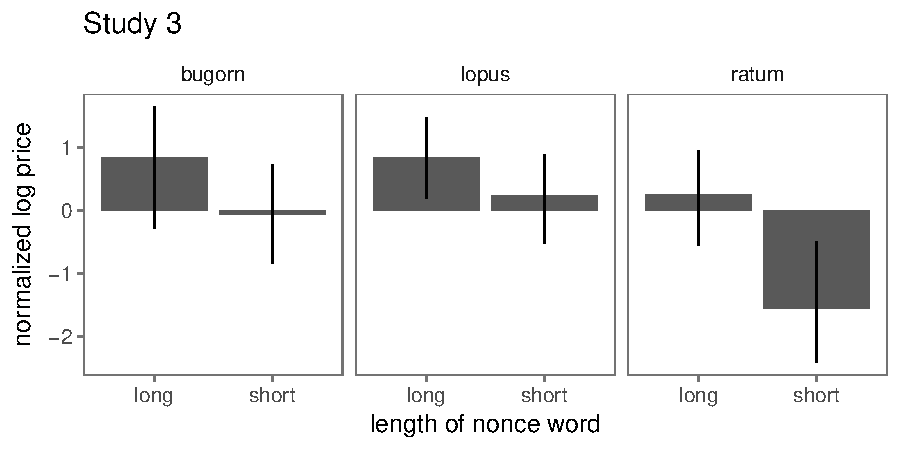
\includegraphics[width=.5\textwidth]{images/plot_study3_A.pdf}
\end{center}
\caption{In Study \hyperref[sec:study3]{3}, we found a significant effect of length for all novel intensifiers.} 
\label{fig:plot_study3_barplot}
\end{figure}

\begin{figure}[hbt]
\begin{center}
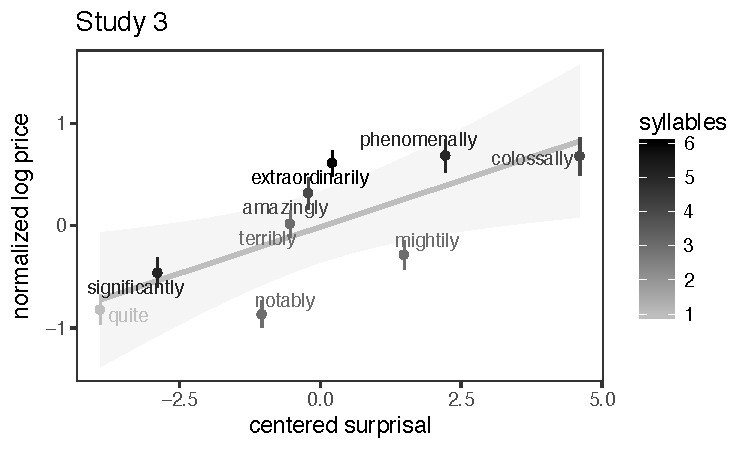
\includegraphics[width=0.5\textwidth]{images/plot_study3_B.pdf}
\end{center}
\caption{In Study \hyperref[sec:study3]{3}, we replicated our findings from Study \hyperref[sec:study1a]{1a}.}
\label{fig:plot_study3_scatter}
\end{figure}

\subsubsection{Results}

In our analysis of novel intensifiers, we found a significant effect of length condition ($b=0.538$, $t=2.757$, $p=0.0002$), indicating that people interpret a longer intensifier as stronger, even for novel intensifiers with no conventional meaning (Figure \ref{fig:plot_study3_barplot}).

Replicating our findings from Study \hyperref[sec:study1a]{1a}, we found significant main effects of surprisal ($b=0.14,t(7.2)=2.49,p=0.0407$) but no significant effect of syllable length ($p=0.0846$) (Figure \ref{fig:plot_study3_scatter}). In likelihood ratio test, we found that the full model was a better fit than the model with surprisal only ($\chi^2(8)=8.296,p=0.0403$) and the model with length only ($\chi^2(8)=39.194,p<0.0005$). Residualizing each regressor with respect to one another, we again found qualitatively similar effects to Studies \hyperref[sec:study1a]{1a} and \hyperref[sec:study1b]{1b}, with a significant effect of surprisal when residualized by length ($b=0.14,t(7.2)=2.49,p=0.0407$) and no significant effect of length when residualized by surprisal ($p=0.085$).

We observe that, numerically, average responses for \w{ratumly} were much lower than all the other intensifiers used in Study \hyperref[sec:study3]{3}.
In a post-hoc regression with fixed effects for the novel adverb roots (\w{ratum/other}=2/-1, \w{lopus/bugorn}=1/-1), we found a significant difference between \w{ratum} and the other roots ($b=-0.56,t(23)=-2.60,p=0.0160$) and no significant difference between the remaining roots ($p=0.759$).
The very low rankings for the root \w{ratum} suggest possible additional effects of form that we have not captured with length in syllables alone.
% \eb{, though we observe that, numerically,
% average responses for \w{ratumly} were much lower than the other intensifiers used in Experiment 3.}
%, and average responses for \w{tupabugornly} were highest.
% The rest of the novel intensifiers had average ratings within the range of the attested intensifiers.

Full results for Study \hyperref[sec:study3]{3} are presented in Appendix \ref{app:3}.

\subsection{Study 4 \label{sec:study4}}

In Study~\hyperref[sec:study4]{4} we again show that longer novel intensifiers are interpreted as having stronger meanings, this time for an additional adjective, using our dependent measure from Study~\hyperref[sec:study2]{2}.

\subsubsection{Methods}

\paragraph{Participants}
60 participants with US IP addresses were recruited through Amazon's Mechanical Turk and paid \$0.16 for their participation. 3 participants were excluded from the analysis for admitting that they did not think they followed the instructions in a post-experiment survey.

\paragraph{Items}

In Study \hyperref[sec:study4]{4}, each participant saw exactly one of two adjectives (\w{expensive} or \w{tall}, varied between participants) with the set of intensifiers from Study \hyperref[sec:study3]{3}. This set included 9 context/filler words and one novel intensifier, which we varied between participants.

\paragraph{Procedure%\footnote{A demo of Study \hyperref[sec:study4]{4} can be found at \url{http://cocolab.stanford.edu/links_for_papers/bennett2017extremely/experiments/Study4/.}}
}

Except for the narrower set of items, noted above, Study \hyperref[sec:study4]{4} was identical to Study \hyperref[sec:study2]{2}. 

As in Study \hyperref[sec:study2]{2}, adjective phrases for each intensifier-adjective pairing were initialized on the left in a random order.

\subsubsection{Analysis}

For the novel intensifiers, we ran a cumulative logit model on the rankings (relative to the filler intensifiers) that participants gave to the novel intensifier.

As in Study \hyperref[sec:study3]{3}, we also ran such a model with regressors for the word stem (or ``root'').

With our filler intensifiers for Study \hyperref[sec:study4]{4} we again ran a ranked order logit model (re-ranking to ignore novel intensifiers) to confirm effects of syllable length and surprisal.

\subsubsection{Results}

In the cumulative logit model, we found a significant effect of length condition ($b=0.7039, z=-2.79, p=0.0054$).

When we included a regressor for the root of the novel intensifier, we did not find a significant difference between participants' relative rankings for \w{ratum} and other roots ($p=0.110$) or between the other two roots ($p=0.304$).

Rankings for novel intensifiers had much higher variance than rankings for attested intensifiers, since we had many fewer rankings for the novel intensifiers (which varied between participants) than for the attested ones (which every participant saw once). The novel intensifier \w{ratumly} was again on average ranked as less strong than any other intensifier, but the highest-ranked novel intensifiers (\w{gaburatumly} and \w{tupabugornly}) were on average ranked below the highest-ranked attested intensifiers (\w{colossally}, \w{phenomenally}, \w{extraordinarily}, and \w{amazingly}).

For the filler items, we replicated our findings from Study \hyperref[sec:study2]{2}, showing significant effects of both surprisal ($b=0.447,t=13.879,p<0.0005$)
and syllable length ($b=0.581,t=10.738,p<0.0005$) on the order in the list that participants chose for the intensifiers (see Figure \ref{fig:plot_study4}).
In likelihood ratio tests, we again found that length alone ($\chi^2(1)=231.574,p<0.0005$) or surprisal alone ($\chi^2(1)=130.33,p<0.0005$) accounted for the data less well than the full model.
As in Study  \hyperref[sec:study2]{2}, residualized surprisal was significant ($b=0.447,t=13.879,p<0.0005
 $) and residualized length was also significant ($b=0.581,t=10.738,p<0.0005$).
This replication is perhaps unsurprising, since we chose intensifiers to cover the full range of surprisal and syllable lengths.

Full results for Study  \hyperref[sec:study4]{4} are presented in Appendix \ref{app:4}.

\begin{figure}[hbt]
\begin{center}
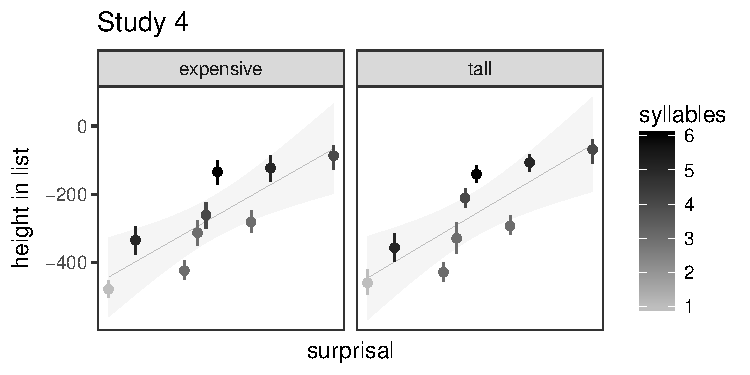
\includegraphics[width=0.5\textwidth]{images/plot_study4.pdf}
\end{center}
\caption{In Study \hyperref[sec:study4]{4}, we replicated our finding from Experiment 2: longer and less frequent intensifiers are ranked higher than shorter and more frequent ones.}
\label{fig:plot_study4}
\end{figure}

\subsection{Discussion}
Overall, in Studies \hyperref[sec:study3]{3} and \hyperref[sec:study4]{4} we found that word length in syllables is a significant predictor of interpretation strength for novel intensifiers.
These novel intensifiers have no established meaning, so the relationship between their length and strength cannot be a direct consequence of the lexicon becoming more efficient over time.
This result is consistent with the hypothesis that participants are inferring the meanings of the novel intensifiers pragmatically, as in the M-implicature account sketched above.

Alternatively, it could be that participants have learned a general relationship between length and meaning of intensifiers in English, and are utilizing this meta-linguistic knowledge to interpret the new words they encounter.

This meta-linguistic hypothesis is less parsimonious than the pragmatic hypothesis, since the pragmatic hypothesis relies only on mechanisms (M-implicature) that we know to be involved in other examples of language understanding (e.g. as in the ``I got the car to start'' example above).
It builds on previous formal models of adjective meaning and informal models of intensifier meaning, generalizing to a wide range of intensifiers.

Whether due to a process of M-implicature or meta-linguistic knowledge, these results demonstrate that the relationship between word cost and meaning is not merely a static, gradual result of language evolution---interpreted meaning of intensifiers depends on length in an active, dynamic way.
